\newpage
\chapter{Пакетна организация, променливи, основни математически операции в R и типове данни}
\label{chapter02}
\thispagestyle{empty}

Най-голямата сила на продукта R се дължи на хилядите пакети\index{пакети} (софтуерни приставки), създадени от безброй потребители на продукта. Наличните пакети покриват цялата област на статистиката и статистическата обработка на данни. 

Под пакет се разбира софтуерна библиотека от предварително написан програмен код, който има за цел да реши определена задача или група от задачи. Тъй като продуктът R е една отворена система, е важно да се има предвид, че не всички пакети са с еднакво качество. Една част от пакетите са изключително професионално написани, устойчиви са на некоректно използване и имат добра база от поддържащи ги потребители. В същото време друга част от пакетите са създадени с голяма доза добри намерения, но работят бавно, дават дефекти или просто не вършат това, за което са създадени. Голяма част от пакетите са написани от статистици за статистици и това може да доведе до някои странни въпроси при част от потребителите, особено при хора, идващи от индустрията за производство на софтуер.

Настоящото учебно помагало представя само най-основните пакети, достатъчни да бъде изложен материалът свързан с базовите познания по R. Опит да бъдат разгледани всички пакети е непосилен за едно издание, най-вече защото броят и видът на пакетите постоянно се променя.

\section{Инсталиране на пакети}

Съществуват различни начини за инсталиране на пакети в R като най-използваният от тях е чрез команда в конзолата на пакета R.

\begin{figure}[h!]
  \centering
  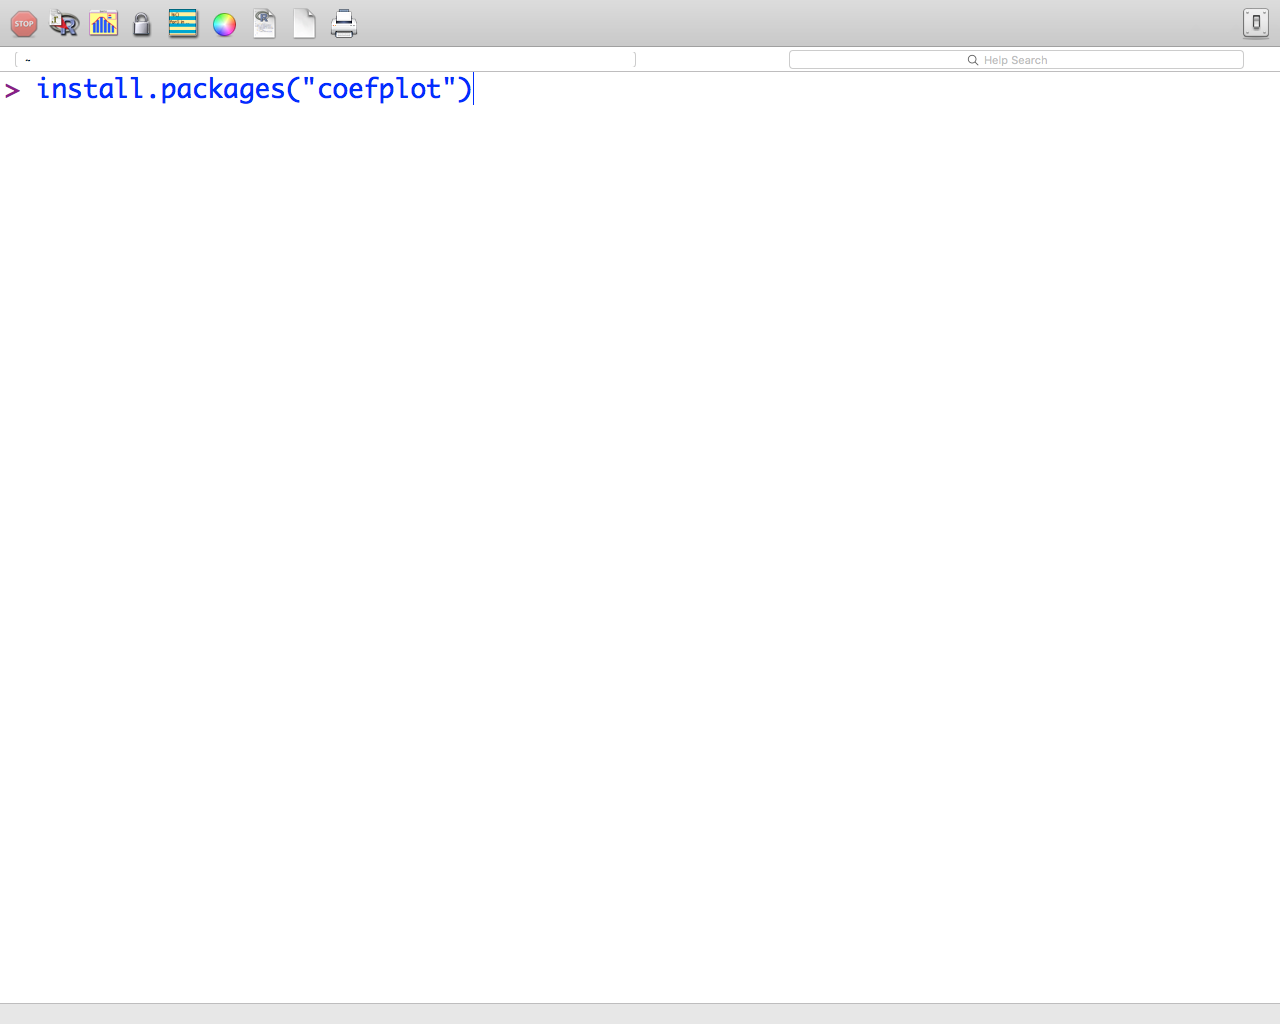
\includegraphics[width=1.0\linewidth]{pic0014}
  \caption{Команда за инсталиране на пакета coefplot}
\label{figure0014}
\end{figure}
\FloatBarrier

За да започне инсталирането на пакет (в случая coefplot) е достатъчно да се изпише командата от Фиг. \ref{figure0014}, със съответното име на пакета като неин параметър.

\begin{figure}[h!]
  \centering
  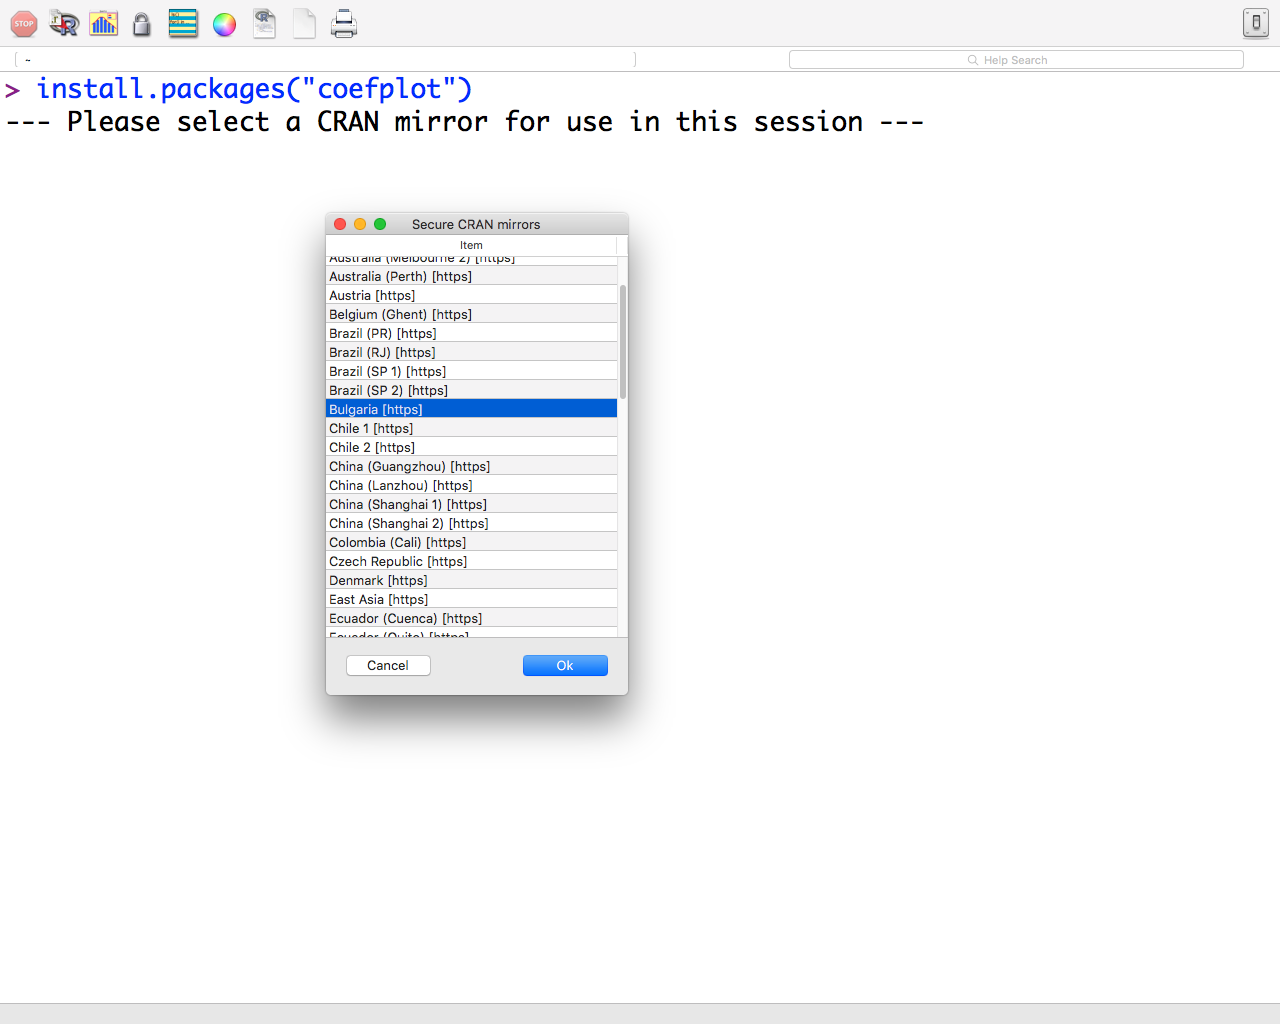
\includegraphics[width=1.0\linewidth]{pic0015}
  \caption{Избор на сървър за изтегляне на пакета}
\label{figure0015}
\end{figure}
\FloatBarrier

Следва избор на сървър за изтегляне на пакета (Фиг. \ref{figure0015}). Разумна стратегия е да се избират сървъри, които териториално се намират в близост до мястото, от което се работи. Това би осигурило малко по-голяма скорост на връзката в Глобалната мрежа.

\begin{figure}[h!]
  \centering
  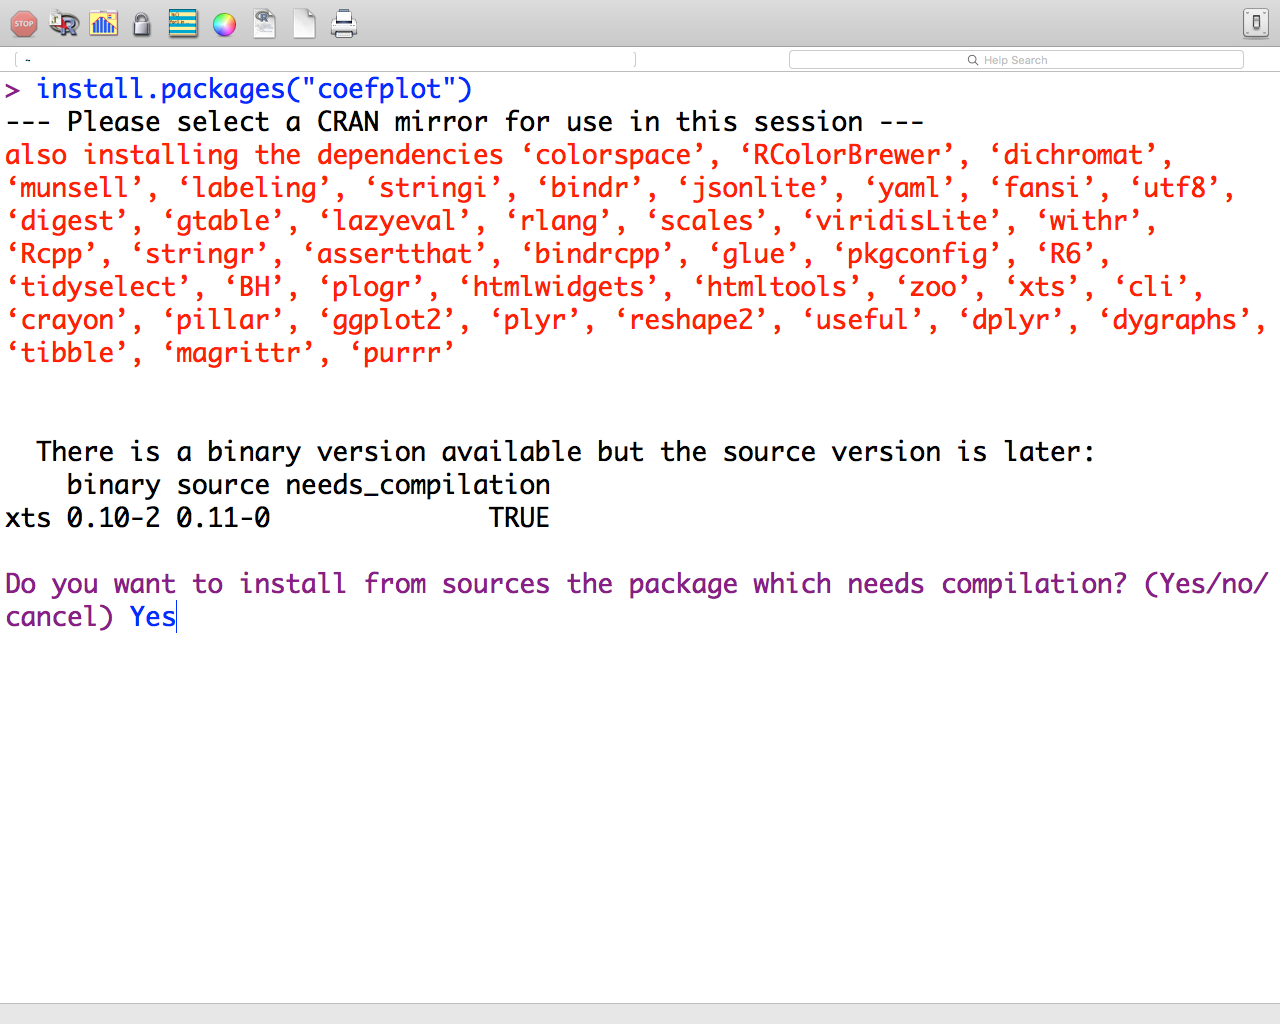
\includegraphics[width=1.0\linewidth]{pic0016}
  \caption{Зависимости между пакетите}
\label{figure0016}
\end{figure}
\FloatBarrier

Често срещан случай е един пакет да има функционална зависимост от други пакети (Фиг. \ref{figure0016}). В такава ситуация е необходимо всички нужни пакети също да бъдат инсталирани. Стратегията при разработка на пакети е те да бъдат предлагани в компилиран (бинарен) вид, но понякога най-новите версии са под формата на програмен код и тогава потребителят има възможност да избере между бинарната версия или версията с програмен код.

\begin{figure}[h!]
  \centering
  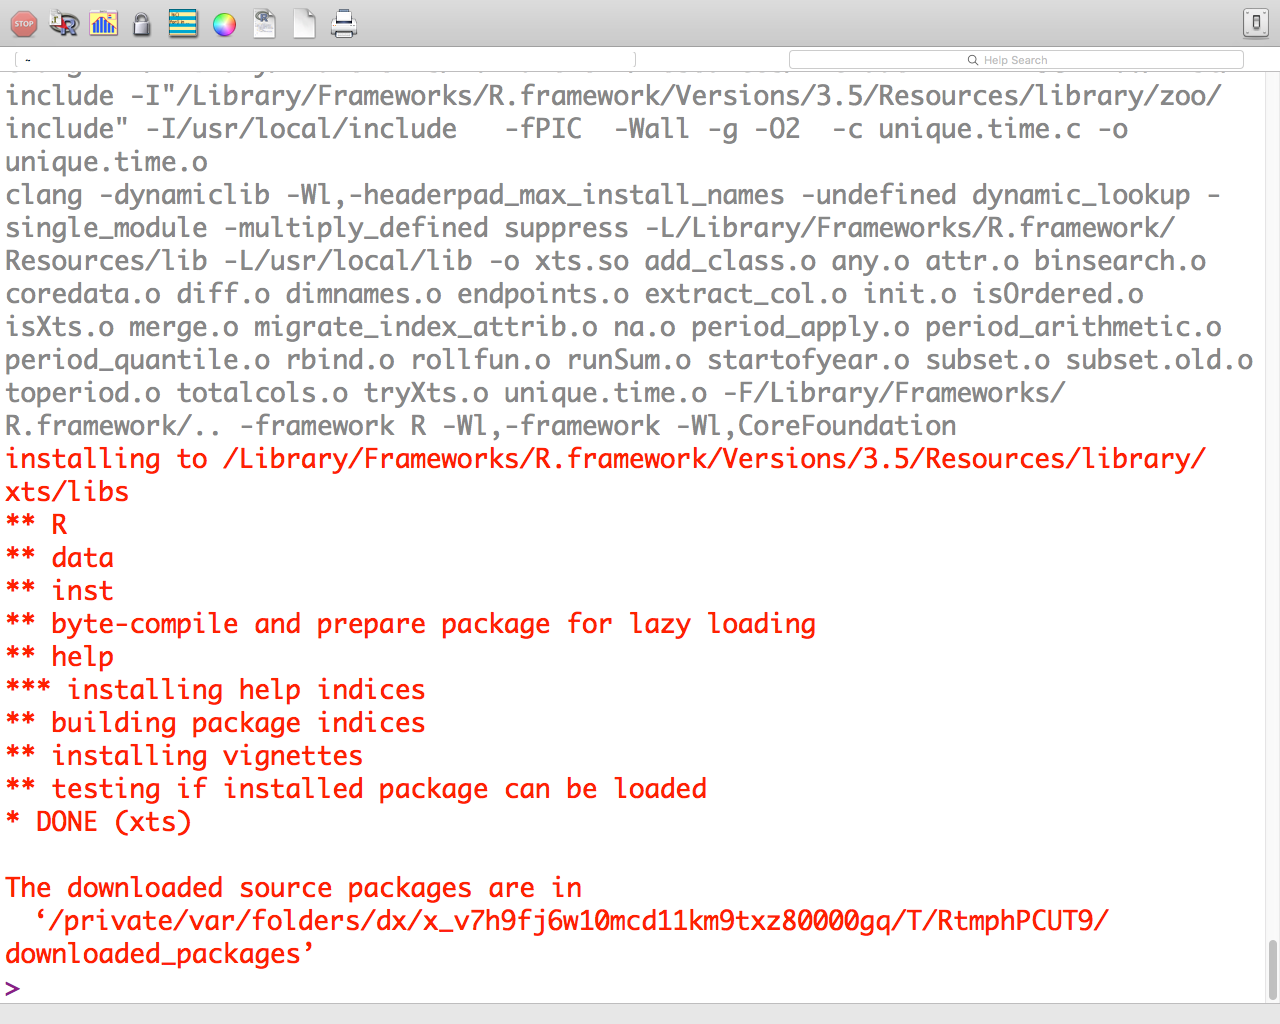
\includegraphics[width=1.0\linewidth]{pic0017}
  \caption{Резултат от инсталацията на пакета}
\label{figure0017}
\end{figure}
\FloatBarrier

Инсталацията на пакета приключва с подробен списък, съдържащ описание на извършените операции (Фиг. \ref{figure0017}).

\begin{figure}[h!]
  \centering
  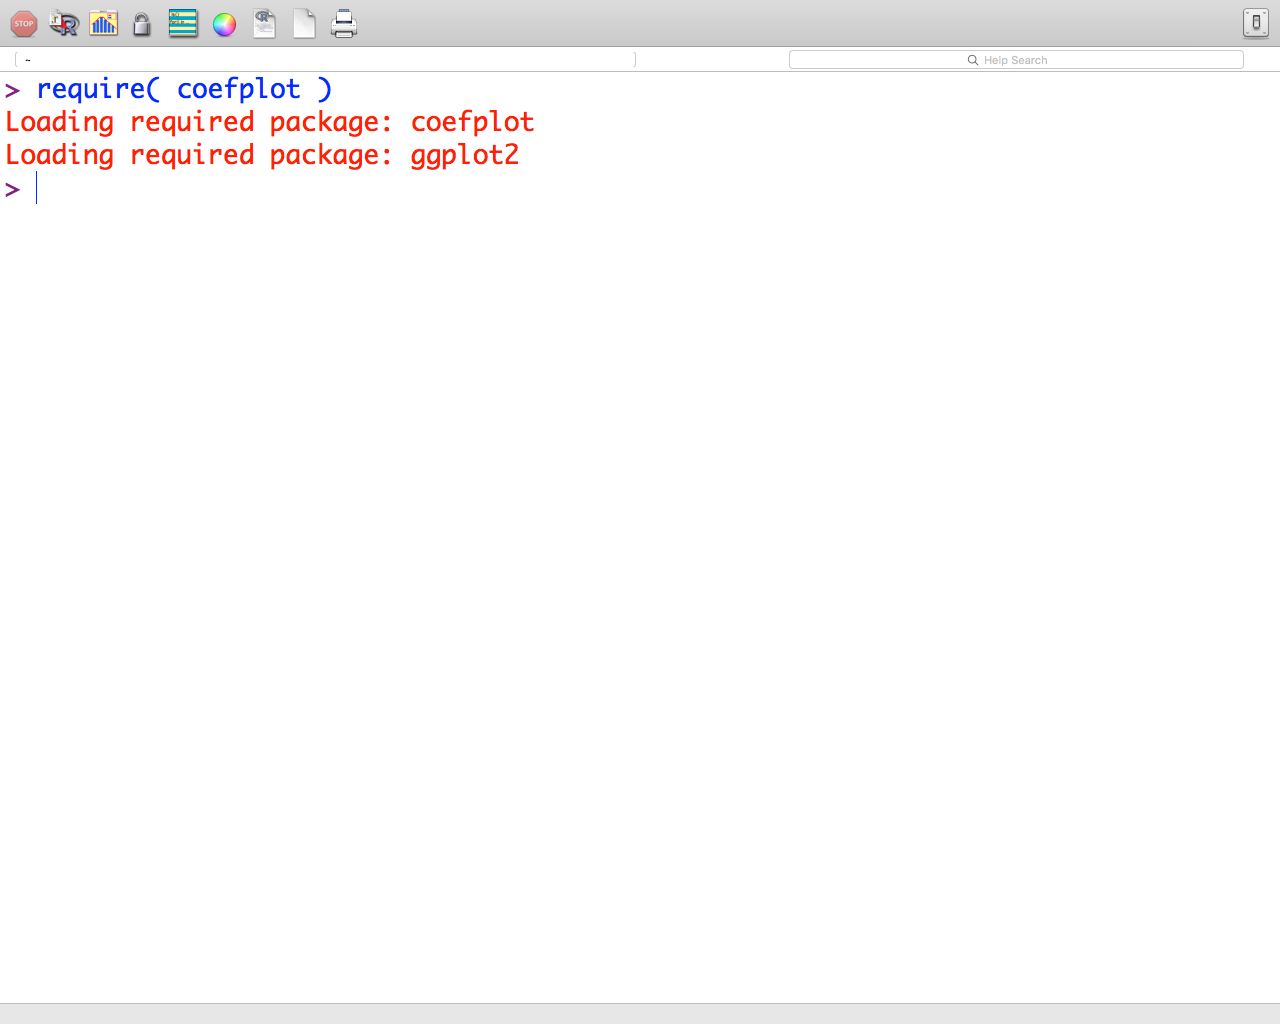
\includegraphics[width=1.0\linewidth]{pic0018}
  \caption{Зареждане на пакета coefplot}
\label{figure0018}
\end{figure}
\FloatBarrier

Дали пакетът е надлежно инсталиран може да се провери с командата require (Фиг. \ref{figure0018}), която зарежда пакета в паметта.

Съществува възможност пакетите да се инсталират под формата на програмен код, директно от хранилищата за програмен код, но за тази цел са нужни подходящите компилатори (най-често C/C++ и Fortran), както и по-задълбочени умения по програмиране. В редки случаи се налага инсталиране на пакета от ZIP файл. При такава ситуация е важно предварително да бъдат инсталирани всички пакети, от които инсталирания пакет зависи.

Премахване на инсталирани пакети става с помощта на командата remove.packages, на която се подава вектор с имената на пакетите, които трябва да бъдат премахнати.

\section{Зареждане на пакети}

За да бъдат използвани пакетите не е достатъчно те да бъдат инсталирани, необходимо е с команда да бъдат включени в текущата сесия от изчисления. R предлага две команди за зареждане на пакети – library и require. И двете изпълняват едно и също нещо – зареждат пакета в общата памет. Разликата е, че require връща TRUE, ако зареждането е било успешно и FALSE при неуспех. Тази възможност е полезна в редките случаи, когато пакетът се зарежда от програмния текст на функция. Подобна практика не е препоръчителна, но R дава такава възможност. И двете функции получават като параметър името на пакета, със или без кавички. Пакетите се зареждат еднократно и остават налични през цялата сесия от изчисления или докато изрично не бъдат премахнати от общата памет.

\begin{figure}[h!]
  \centering
  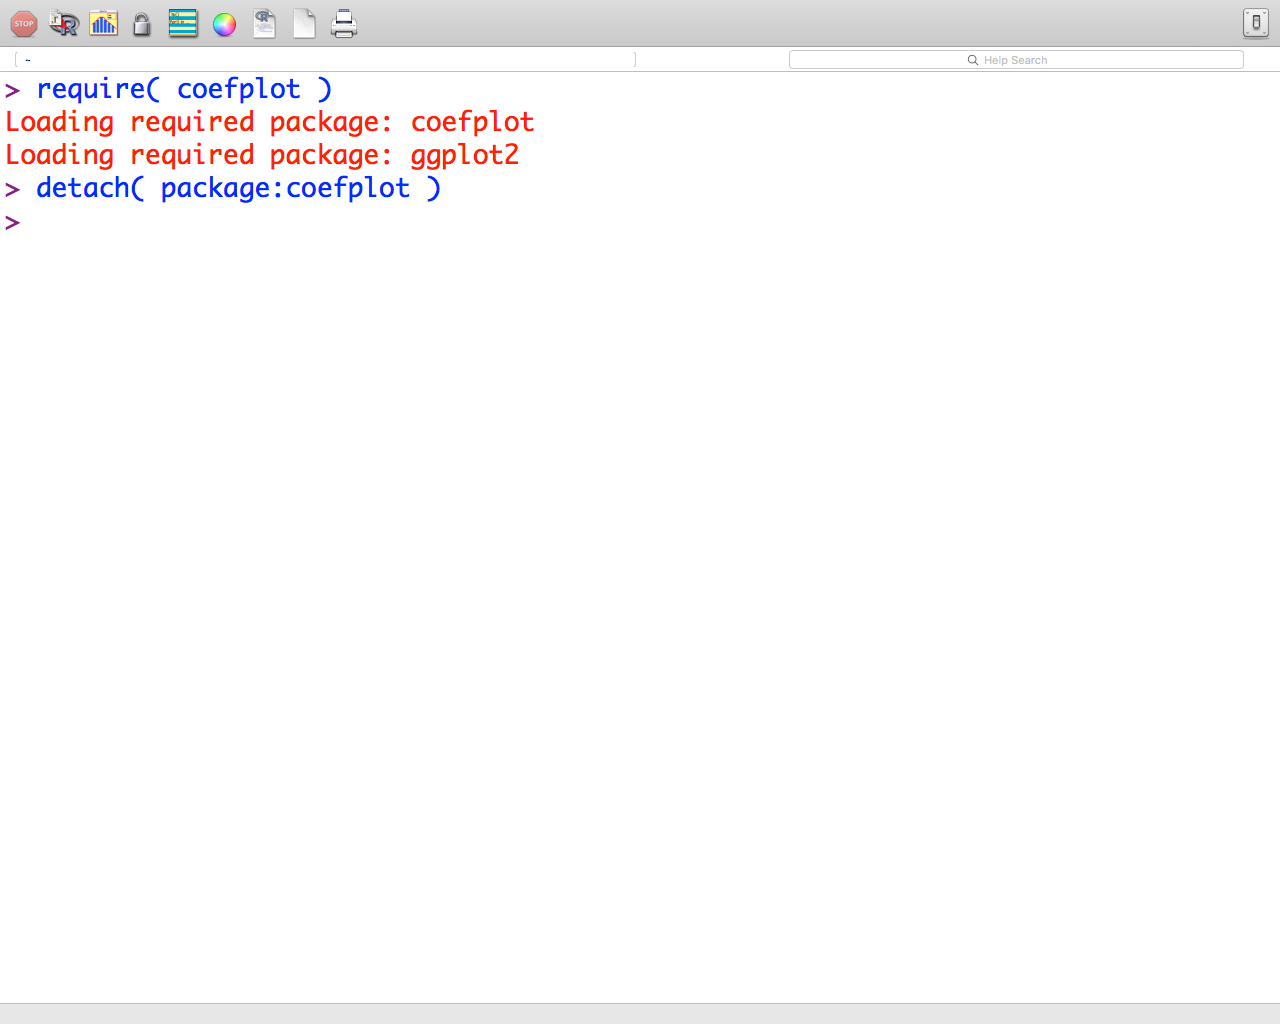
\includegraphics[width=1.0\linewidth]{pic0019}
  \caption{Премахване на пакета coefplot от общата памет}
\label{figure0019}
\end{figure}
\FloatBarrier

Премахването на пакет от общата памет става с командата detach (Фиг. \ref{figure0019}). Същественото при тази команда е, че преди името на пакета се записва думата package.

Тъй като пакетите се разработват основно на доброволни начала, нерядко се случва в различни пакети да има едноименни функции. При подобна колизия на имената решението е да се приложи операцията за принадлежност – двойно двоеточие (::). Когато бъде използвана операцията за принадлежност,  може да не се зарежда пакетът, към който принадлежи функцията.

\section{Основни математически операции}

R позволява да се извършват сложни математически пресмятания\index{математически операции}, но също така може да се използва и за базови математически изчисления. 

\begin{figure}[h!]
  \centering
  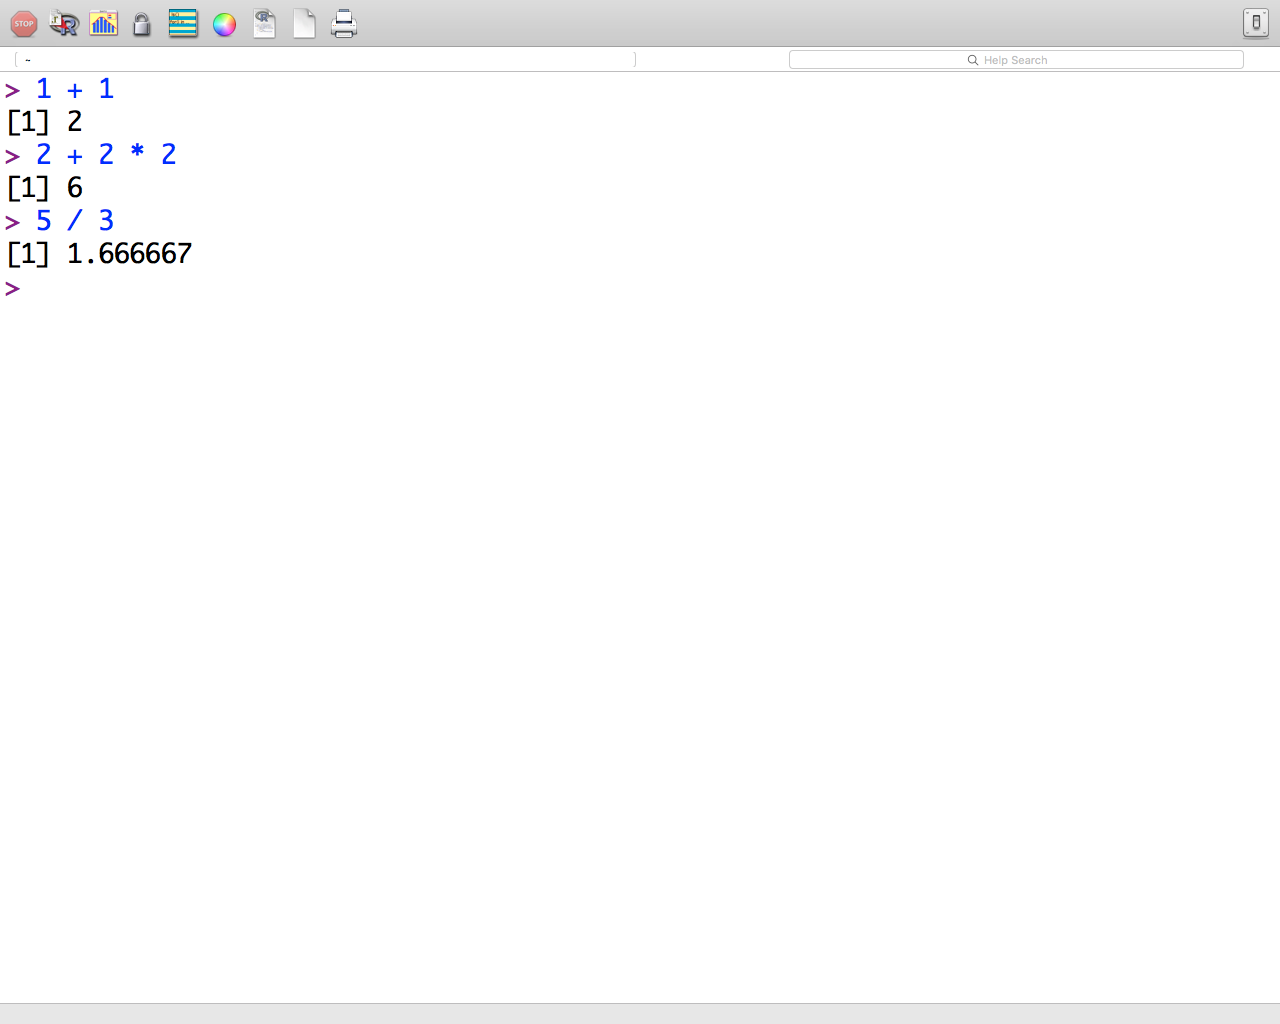
\includegraphics[width=1.0\linewidth]{pic0020}
  \caption{Примерни аритметични операции}
\label{figure0020}
\end{figure}
\FloatBarrier

Най-базовите математически операции са събирането, изваждането, умножението и делението\index{аритметични операции}. Тези операции се изпълняват в R както е показано на Фиг. \ref{figure0020}. Пресмятанията в R се състоят от операции и операнди. Когато няколко операции бъдат обединени, чрез операндите си, се получава математически израз.

\begin{lstlisting}[caption=Събиране, label=listing0001]
1 + 1
\end{lstlisting}

В листинг \ref{listing0001} е демонстрирана операцията за събиране, която има два операнда. Когато става въпрос за математически операции, те имат серия свойства. Като най-съществена характеристика може да се отбележи броят на операндите. Събирането е класически пример за бинарна операция\index{бинарни операции}, тъй като има два операнда (ляв и десен).

\begin{lstlisting}[caption=Унарен минус, label=listing0002]
-5
\end{lstlisting}

В гимназиалния курс по математика не се споменава наличието на унарен плюс, макар и да се учи за унарен минус\index{унарни операции} (Листинг \ref{listing0002}). Унарните плюс и минус променят значението на операнда. В примера от листинг \ref{listing0002}, унарният минус променя значението на числото пет от положително към отрицателно. Тъй като унарният плюс не променя значението на операнда си, масова практика е знакът на унарния плюс да не се записва, това е нещо, което не е възможно с унарния минус. Освен унарни и бинарни операции в някои езици (например C/C++, Java, C\#, PHP и други) съществува една единствена тернарна операция (?:)\index{тернарна операция}, която има смисъла на условния оператор за преход if.

Както бе споменато по-горе, комбинацията от няколко операции и техните операнди водят до съставянето на математически израз\index{математически изрази} (Листинг \ref{listing0003}).

\begin{lstlisting}[caption=Аритметичен израз с две събирания, label=listing0003]
2 + 2 + 2
\end{lstlisting}

Тъй като съвременните изчислителни машини са организирани по такъв начин, че процесорът да извършва само една математическа операция на един такт от пресмятането, става актуален въпросът коя от операциите ще бъде изпълнена първа и коя втора, при положение, че операциите са с еднакъв приоритет. Тъй като в англосаксонската писмена система е прието да се пише и чете от ляво на дясно, то множество математически операции се изпълняват от ляво на дясно. Това се нарича лява асоциативност\index{лява асоциативност} и събирането е точно от тази група операции.

\begin{lstlisting}[caption=Израз за каскадно присвояване, label=listing0004]
a = b = 2
\end{lstlisting}

В гимназиалната математика символът равно се използва за проверка на идентичността между двата операнда, но в компютърните езици символът за равенство има смисъл на операция за присвояване. Това означава, че десният операнд бива присвоен като стойност на левия операнд. При съставянето на математически израз с каскада от присвоявания няма друг вариант, освен първо най-десният операнд да бъде изпълнен и едва накрая най-левият. Това се нарича дясна асоциативност\index{дясна асоциативност} и се използва при значително малък брой от математическите операции.

\begin{lstlisting}[caption=Контекстна зависимост на операциите, label=listing0005]
"abc" + "def"
2 + 2
\end{lstlisting}

Следващата важна характеристика на математическите операции е тяхната контекстна зависимост\index{контекстна зависимост на операциите}. В множество езици събирането на символни низове води до конкатенация (не и в R), докато събирането на числа води до резултат от числено събиране (Листинг \ref{listing0005}).

\begin{lstlisting}[caption=Контекстна зависимост на операцията за делене, label=listing0006]
5 / 3
5.0 / 3.0
\end{lstlisting}

В множество програмни езици (с изключение на R) операцията за деление е контекстно зависима (Листинг \ref{listing0006}). Когато и двата операнда са цели числа, резултатът е целочислено деление, а когато поне един от операндите е дробно число, то резултатът е дробно число.

\begin{lstlisting}[caption=Приоритет на операциите, label=listing0007]
2 + 2 * 2
\end{lstlisting}

Когато в един математически израз участва повече от една операция с еднаква асоциативност, от значение става приоритетът\index{приоритет на операциите} на всяка от тях. Най-често даваният пример е събирането и умножението (Листинг \ref{listing0007}). В случая първо се извършва умножението, тъй като е по-високо приоритетно, а едва след това събирането.

\begin{lstlisting}[caption=Смяна на приоритета, label=listing0008]
(2 + 2) * 2
\end{lstlisting}

В компютърните езици кръглите скоби имат смисъла на операция за промяна на реда, по който ще се извърши пресмятането с цел смяна на приоритета (Листинг \ref{listing0008}).

Последният съществен признак на операциите е в коя група попадат – аритметични, логически, побитови, за сравнение, за присвояване и други.

\section{Типове и променливи}

Повечето съвременни програмни езици организират работата с информация в групи от променливи\index{променливи}. За разлика от строго типизираните езици, в R не се задава тип на променливата\index{типове данни}. Типът на променливата неявно се определя от стойността, която е присвоена към нея. Това позволява да се присвояват дори обекти или функции и означава, че една и съща променлива може да съдържа данни от различни типове в различни моменти от времето.

\subsection{Създаване на променливи}

Променливата се появява в общата памет веднага след първата операция за присвояване, за което съществува цяла група операции за присвояване (Листинг \ref{listing0009}). Променливите в R могат да съдържат в имената си латинските букви и арабските цифри, също символа точка (.) и подчертавка (\_). Имената на променливите не могат да започват с цифра или с подчертавка и са чувствителни към регистъра на буквите (малки/големи)\index{именуване на променливи}.

\begin{lstlisting}[caption=Операции за присвояване, label=listing0009]
a = 1
b <- 2
c = d = 3
e <- f <- 4
assign("g", 5)
a += 6
b -= 7
\end{lstlisting}

Стрелка на ляво (<-) служи за присвояване в R, но в повечето конвенционални програмни езици не присъства\index{операции за присвояване}.

\begin{lstlisting}[caption=Алтернативи за операцията присвояване, label=listing0010]
median(x = 1:10)
median(x <- 1:10)
\end{lstlisting}

Разликата между двете операции си проличава най-ясно при извикването на функции с аргументи (Листинг \ref{listing0010}). В първия случай променливата x не остава в глобалната памет, а изчезва, докато при втория случай променливата x остава в глобалната памет след извикването.

Добра практика е за имена на променливите да се избират съществителни имена, а не еднобуквени имена или съкращения.

\subsection{Премахване на променливи}

\begin{lstlisting}[caption=Премахване на променливи от глобалната памет, label=listing0011]
rm( a )
rm( list=ls() )
\end{lstlisting}

Премахването на променлива от общата памет става с командата rm (Листинг \ref{listing0011}). За да се почисти цялата глобална памет се дава списък с всички променливи, налични в глобалната памет. Въпреки че R извиква Garbage Collector-а, на определени интервали от време с командата gc() може да бъде отправена пряка заявка за освобождаване на ненужно заетата памет.

\subsection{Дискретно представяне на информацията}

Информацията в съвременните изчислителни машини се представя само с две нива 0 (няма сигнал) и 1 (има сигнал)\index{представяне на информацията}. Това е свързано с факта, че съвременните изчислителни машини използват електричество. Наличието само на две различими нива позволява единствено бинарна логика. Една клетка, която може да съдържа 0 или 1 носи един бит информация. Това количество е крайно недостатъчно за изчисленията, които хората имат нужда да правят. За да се разширят възможностите на бинарната логика се използва принципът на супер позицията. Отделните битове се подреждат един до друг и колкото по-вляво е един бит, толкова по-голяма тежест има. В зората на изчислителната техника, макар и да е имало коментари за 4 битови изчислителни машини, такава никога не е създадена за реална употреба. Изборът пада върху 8 битовите машини, които позволяват кодирането на 256 стойности в една машинна дума. Групата от 8 бита, хората наричат байт. Байт е единицата, която масово се използва в ежедневието, също и кратните ѝ форми за MB (мегабайт), GB (гигабайт) или TB (терабайт). Дължината на машинната дума има пряка връзка с размерността на някои от първите типове данни. При 8 битовите машини, в C компилатора, типът int е 8 бита, при 16 битовите е 16 бита, а при 32 битовите е 32 бита. Подредбата на битовете в байтове позволява да се обозначат положителните числа и в езика C това е типът unsigned int. Тъй като в света, който познаваме отрицателни неща няма, то въвеждането на абстракцията за отрицателни числа е нещо неестествено за изчислителните машини и трябва да се избере някаква семантика за различаване на отрицателните от положителните числа. При числата със знак е прието най-старшият разред да бъде използван за знак. По този начин се получава феноменът +0 и -0 нещо, което не се разглежда в гимназиалния курс по математика. Ако най-старшият разряд е високо ниво, а останалите са в ниско се получава отрицателна нула. Ако всички разряди са ниско ниво, то се получава положителна нула. Ограничеността на машинната дума води до серия ограничения при работата с числа. Най-често срещаният проблем е препълването на разрядната решетка. Това е проблем, който и в наши дни се среща в програмния език Java (Листинг \ref{listing0015}).

\begin{lstlisting}[caption=Грешка от препълване при събиране, label=listing0015]
System.out.println( 2 + 2 );
4
System.out.println( 2_000_000_000 + 2_000_000_000 );
-294967296
\end{lstlisting}

Когато се налага да се извършват пресмятания с много големи числа е важно да не се ползват конвенционалните програмни езици, а софтуерни продукти като Matlab, Mathematica или R.

Светът, който познаваме не съдържа концепцията за дробност. Дори елементарните частици са изградени от по-малки елементарни частици. Причината за това е, че живеем в дискретен, а не в непрекъснат свят. Все пак, човекът е въвел концепцията за дробните числа, така че да извършва пресмятания, които да му позволяват по-ясно разбиране на света. Поради чисто физическата си природа разрядната решетка не може да съдържа дробни стойности. Представянето на цели числа е възможно чрез принципа на супер позицията, но той не е приложим при дробните числа. Най-лесният начин да се представи едно дробно число е чрез използването на две цели числа – едно за цялата част и едно за дробната част. Такова представяне е чисто схематично, на практика дробните числа в изчислителните машини се представят по IEEE стандарт. Както може да се препълни цялата част, така може да се препълни и дробната част, което води до проблем познат като underflow. Причината е в това, че компютърът не може да отрази понятието за безкрайност, а между две цели числа (например между 0 и 1) има безкрайно много дробни числа. В изчислителната математика е възприето правилото, че отговорни пресмятания никога не се правят в дробни числа, а се търси вариант за пресмятане с цели числа или чрез пакети за символно пресмятане.

Тъй като в изчислителната техника съществуват само сигнали от ниско и високо ниво, то няма как да бъде кодирана информация за букви или текст. Естественият начин за комуникация между човека и машината са точно текстовете. Поради тази причина в изчислителната техника буквите от естествените езици са номерирани по стандартизирани кодови таблици. Две от най-популярните кодови таблици са ASCII и UTF-8. ASCII стандартът е силно ограничен и не позволява кодирането на повечето естествени езици, поради тази причина е създаден стандартът UTF-8 (един от най-разпространените в наше време), който позволява достатъчно икономично да бъдат представени символите от азбуките на познатите естествени езици.

\subsection{Числени стойности}

Условно R спада към групата на безтиповите езици, но всяка променлива вътрешно съхранява информация, която определя типа на данните. Възможни са различни типове данни, но най-използваните са numeric, character (включително символни низове), Date/POSIXct (астрономическо време) и logical (TRUE/FALSE).

\begin{lstlisting}[caption=Проверка за типа на променливата, label=listing0012]
a = 5
class( a )
[1] "numeric"
\end{lstlisting}

С помощта на функцията class (Листинг \ref{listing0012}) може да се провери типът на променливата. Тъй като R основно се използва за изчисления, то най-употребяваният тип данни са числовите данни\index{числени типове}. В този аспект numeric съответства на типовете float и double в другите конвенционални езици за програмиране. Този тип данни се използва за цели и дробни числа, както и за нулата. Това е типът по подразбиране, който се задава на променливата при числено присвояване.

\begin{lstlisting}[caption=Проверка за типа numeric, label=listing0013]
is.numeric( a )
[1] TRUE
\end{lstlisting}

Проверката за numeric типа се извършва както е показано в листинг \ref{listing0013}.

\begin{lstlisting}[caption=Използване на целочислен тип, label=listing0014]
b <- 6L

class( b )
[1] "integer"

is.numeric( b )
[1] TRUE

is.integer( b )
[1] TRUE

is.integer( a )
[1] FALSE
\end{lstlisting}

R допуска използването само на цели числа, чрез типа integer. За да бъде указан типът integer към числото се добавя буквата L (Листинг \ref{listing0014}).

\subsection{Символни низове}

\begin{lstlisting}[caption=Символни низове в R, label=listing0016]
s1 <- "Simple text."
s1
[1] "Simple text."

class( s1 )
[1] "character"

s2 <- factor( "Another simple text." )
s2
[1] Another simple text.
Levels: Another simple text.

class( s2 )
[1] "factor"
\end{lstlisting}

За символни низове\index{символни низове} има два възможни варианта, които са показани на листинг \ref{listing0016}. Символните низове в R са чувствителни към малки и големи букви. Фактор е специален символен низ, който намира приложение при векторите.

\begin{lstlisting}[caption=Дължина на символен низ или числена стойност, label=listing0017]
nchar( s1 )
[1] 12

nchar( s2 )
Error in nchar(s2) : 'nchar()' requires a character vector

nchar( a )
[1] 1
\end{lstlisting}

Дължината на символен низ или числена стойност може да се определи с функцията nchar, която обаче не е приложима за променливите от тип фактор (Листинг \ref{listing0017}).

\subsection{Астрономическо време}

При статистическата обработка на данни много често измерванията се извършват в точно определен момент от времето. Това налага наличието на възможности за обработка на астрономическо време\index{типове за астрономическо време}. Работата с астрономическо време носи своите трудности поради множество фактори. От една страна има множество часови зони. Също така различните месеци в годината имат различен брой дни. Някои години се различават по брой дни. В една част от държавите се минава към лятно часово време и зимно часово врем, докато в другите това не се прави.

\begin{lstlisting}[caption=Типове данни за време, label=listing0018]
d1 <- as.Date("1979-04-21")
d1
[1] "1979-04-21"

class( d1 )
[1] "Date"

as.numeric( d1 )
[1] 3397

d2 <- as.POSIXct("1980-02-12 05:25")
d2
[1] "1980-02-12 05:25:00 EET"

class( d2 )
[1] "POSIXct" "POSIXt" 

as.numeric( d2 )
[1] 319173900
\end{lstlisting}

В R най-често използваните типове за астрономическо врем са Date и POSIXct (Листинг \ref{listing0018}). Типът Date съхранява само информацията за дата, докато типът POSIXct съхранява информация за датата и за часа. Вътрешното представяне на Date е брой дни от 1 януари 1970 година, а вътрешното представяне на POSIXct е брой секунди от 00:00:00 на 1 януари 1970 година. Тъй като боравенето с информация за астрономическо време може да бъде относително сложно, то за тази цел са налични два помощни пакета - lubridate и chron.

\subsection{Логически стойности}

Логическият тип данни\index{логически тип данни} е също често използван и е в групата на простите типове данни. Променливите съдържат стойности FALSE или TRUE. На предефинираните константи са присвоени числени стойности 0 за FALSE и 1 за TRUE.

\begin{lstlisting}[caption=Логически тип данни, label=listing0019]
x1 <- TRUE
x1
[1] TRUE

class( x1 )
[1] "logical"

is.logical( x1 )
[1] TRUE

as.numeric( x1 )
[1] 1

x2 <- F
x2
[1] FALSE

class( x2 )
[1] "logical"

is.logical( x2 )
[1] TRUE

as.numeric( x2 )
[1] 0
\end{lstlisting}

Освен пълното изписване на булевите стойности, може да се използват променливите T и F, но те не са препоръчителни, тъй като могат да бъдат предефинирани и това да доведе до сериозни логически грешки (Листинг \ref{listing0019}).

\begin{lstlisting}[caption=Операции за сравнение, label=listing0020]
2 == 3
[1] FALSE

5 != 6
[1] TRUE

"Peter" == "Ivan"
[1] FALSE
\end{lstlisting}

Логическият тип данни най-често се получава в следствие на операциите за сравнение (Листинг \ref{listing0020}).

\section*{Заключение}

В тази глава са разгледани основните принципи за работа с пакети, работата с променливи, най-съществените операции с данни и някои от базовите типове данни.
